%----------------------------------------------%
%                                              %
% Title:  Linux device drivers explained       %
% Author: Giuseppe Calderaro                   %
% Date:   29th October 2009                    %
%                                              %
%----------------------------------------------%

% Latex document class
\documentclass{beamer}
\usepackage{beamerthemeshadow}
\usepackage{listings}
\lstset{language=C}
\setbeamertemplate{navigation symbols}{}
\usetheme{Berkeley}
\beamersetuncovermixins{\opaqueness<1>{25}}{\opaqueness<2->{15}}

% Document start
\begin{document}
\title{Linux Device Drivers explained}
\author{Giuseppe Calderaro}
\institute[http://www.imgtec.com/]{Imagination technologies ltd.}
\date{29th October 2009}

% Slide: 1
\frame{\titlepage}

% Slide: 2
\frame{\frametitle{Table of contents}\tableofcontents}

%% LINUX SYSTEM ARCHITECTURE
% Slide: 3
\section{Linux system architecture}
\subsection{Linux system architecture}
\frame{\frametitle{Linux system architecture}
  \begin{columns}
    \begin{column}{10cm}
      \begin{figure}
        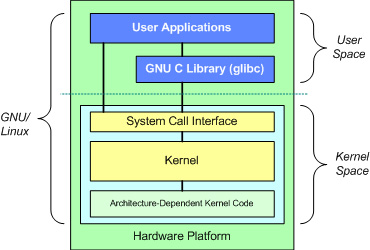
\includegraphics[scale=0.75]{arch1.eps}
        \caption{Linux system architecture}
      \end{figure}
    \end{column}
  \end{columns}
}

% Slide: 4
\subsection{Linux kernel architecture}
\frame{\frametitle{Linux kernel architecture}
  \begin{columns}
    \begin{column}{3cm}
      \begin{figure}
        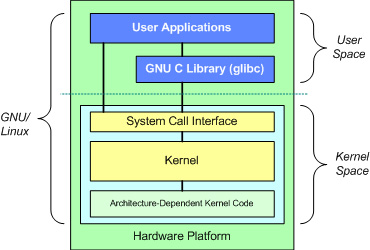
\includegraphics[scale=0.35]{arch1.eps}
        \caption{\tiny{Linux system architecture}}
      \end{figure}
    \end{column}
    \begin{column}{7cm}
      \begin{figure}
        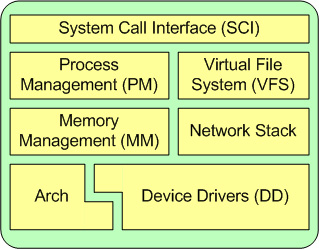
\includegraphics[scale=0.65]{arch2.eps}
        \caption{Linux kernel architecture}
      \end{figure}     
    \end{column}
  \end{columns}
}

%% BUILDING AND RUNNING MODULES
% Slide: 5
\section{Building and running modules}
\subsection{A polite module...}
\frame{\frametitle{A polite module...}
  \makebox{
    \scriptsize{
      \lstinputlisting{example.c}
    }
  }
}

% Slide: 6
\subsection{...and his Makefile}
\frame{\frametitle{...and his Makefile}
  \makebox{
    \scriptsize{
      \lstinputlisting{Module_Makefile}
    }
  }
}

%% DEBUGGING TECHNIQUES
% Slide: 7
\section{Debugging techniques}
\subsection{printk}
\frame{\frametitle{printk}
  Log level strings:
}

% Document end
\end{document}
